\section{Modélisation}

	L'analyse préalable nous permet à présent d'avoir une vision plus précise des fonctionnalités de notre programme en vue de réaliser son diagramme de classe. Pour simplifier la modélisation et permettre une plus grande modularité de nos classes nous avons voulu utiliser un maximum des patrons de conceptions. 

	\subsection{patron de Conception}

		\subsubsection{Monteur : création d'une partie}

		\textbf{Bedbihan} permet aux joueurs de jouer différentes type de parties. Ainsi il existe différentes manières de construire une partie en fonction du type désiré. Néanmoins ces créations passent par des étapes similaires : création de la carte, créations des unités, etc. C'est pourquoi sur  la création de la partie est assurée par le patron de conception \textbf{Monteur}. Ce patron de conception nous permet de séparer la conception de l'objet \emph{Game} de sa représentation. Comme indiqué la sur la FIGURE \ref{fig:builder}, la création de la partie sera dirigé par le \emph{GameCreator} qui utilisera le monteur adéquat en fonction de la situation. Ainsi d'une part on minimise le code en évitant des répétitions et de l'autre on gagne en flexibilité : il sera facile de créer un type de partie différent. 

		\begin{figure}[h]
		\begin{center}
			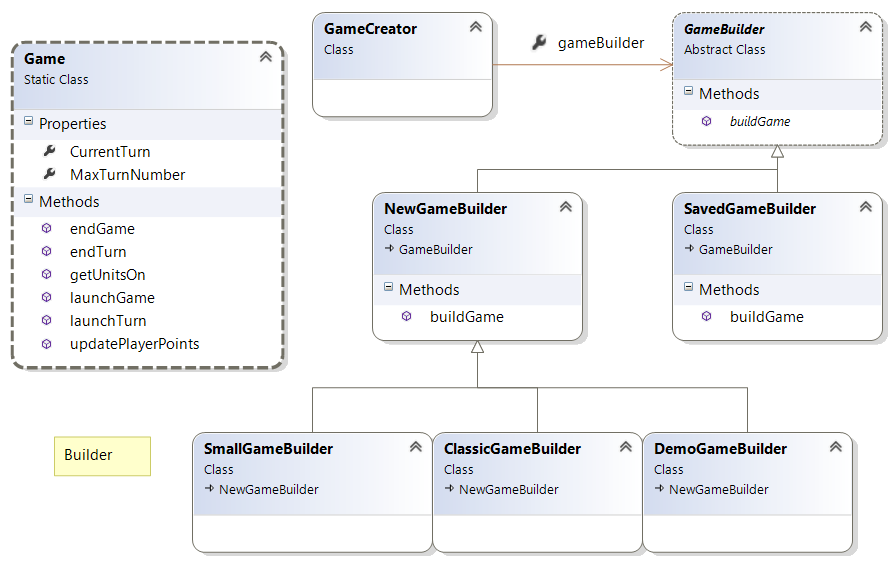
\includegraphics[width=0.5\textwidth]{figure/builder.png}
		\end{center}
		\caption{Création de la partie : patron de conception Monteur}
		\label{fig:builder}
	\end{figure}

		\subsubsection{Fabrique : création de différents peuples}

		\begin{figure}[h]
			\begin{center}
				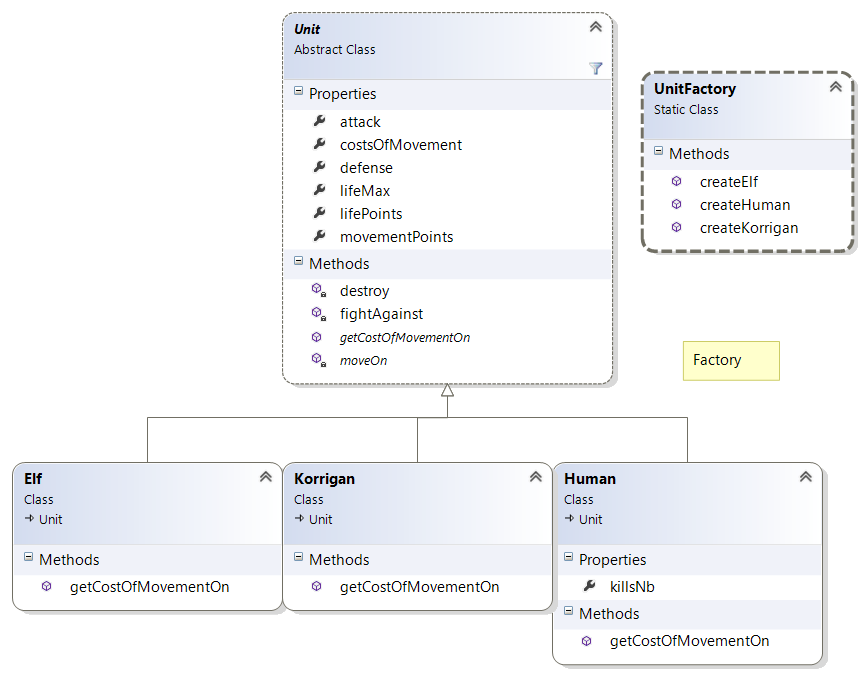
\includegraphics[width=0.5\textwidth]{figure/factory.png}
			\end{center}
			\caption{Création des unités : patron de conception Factory}
			\label{fig:strategy}
		\end{figure}

		Chaque joueur posséde une armée composé d'un certain nombre d'unité d'un même peuple, selon le type de parties. Ces untiés sont soit des Elfs, des humains ou des Korrigans. Cela se traduit, dans notre modélisation, par l'objet \emph{Player} qui posséde une \emph{Faction}, elle même composé d'objets \emph{unité}. l'\emph{unité} est une classe abstraite implémentée par trois classes concretes réprésentants les trois type d'unités disponible. La création de ces unité est assurée par le patron de conception \textbf{Fabrique}. Ce patron de conception nous permettra de créer l'armée adéquate en fonction du peuple choisie par le joueur au lancement de la partie. Il asure une modularité du code, car sa fonction \emph{CreateUnit} retourne un type abstrait. Ainsi, l'appelant n'as pas besoin de se préoccuper du type de retour.  A MODIFIER



		\subsubsection{Poids-Mouche : gestion des cases}

		\subsubsection{Stratégie : création des différents type de carte}



		La création des cartes, de tailles fixes mais dont la composition des dalles est implémentée de maniére aléatoire, repose sur le patron de conception \emph{stratégie}. Ce patron de conception nous permet de choisir de manière précise l'algorithme de création de carte désiré. De plus, il permet une grande flexibilité pour définir de nouveaux types de cartes.



	\subsection{Diagramme de classe}


	\begin{figure}
		\begin{center}
			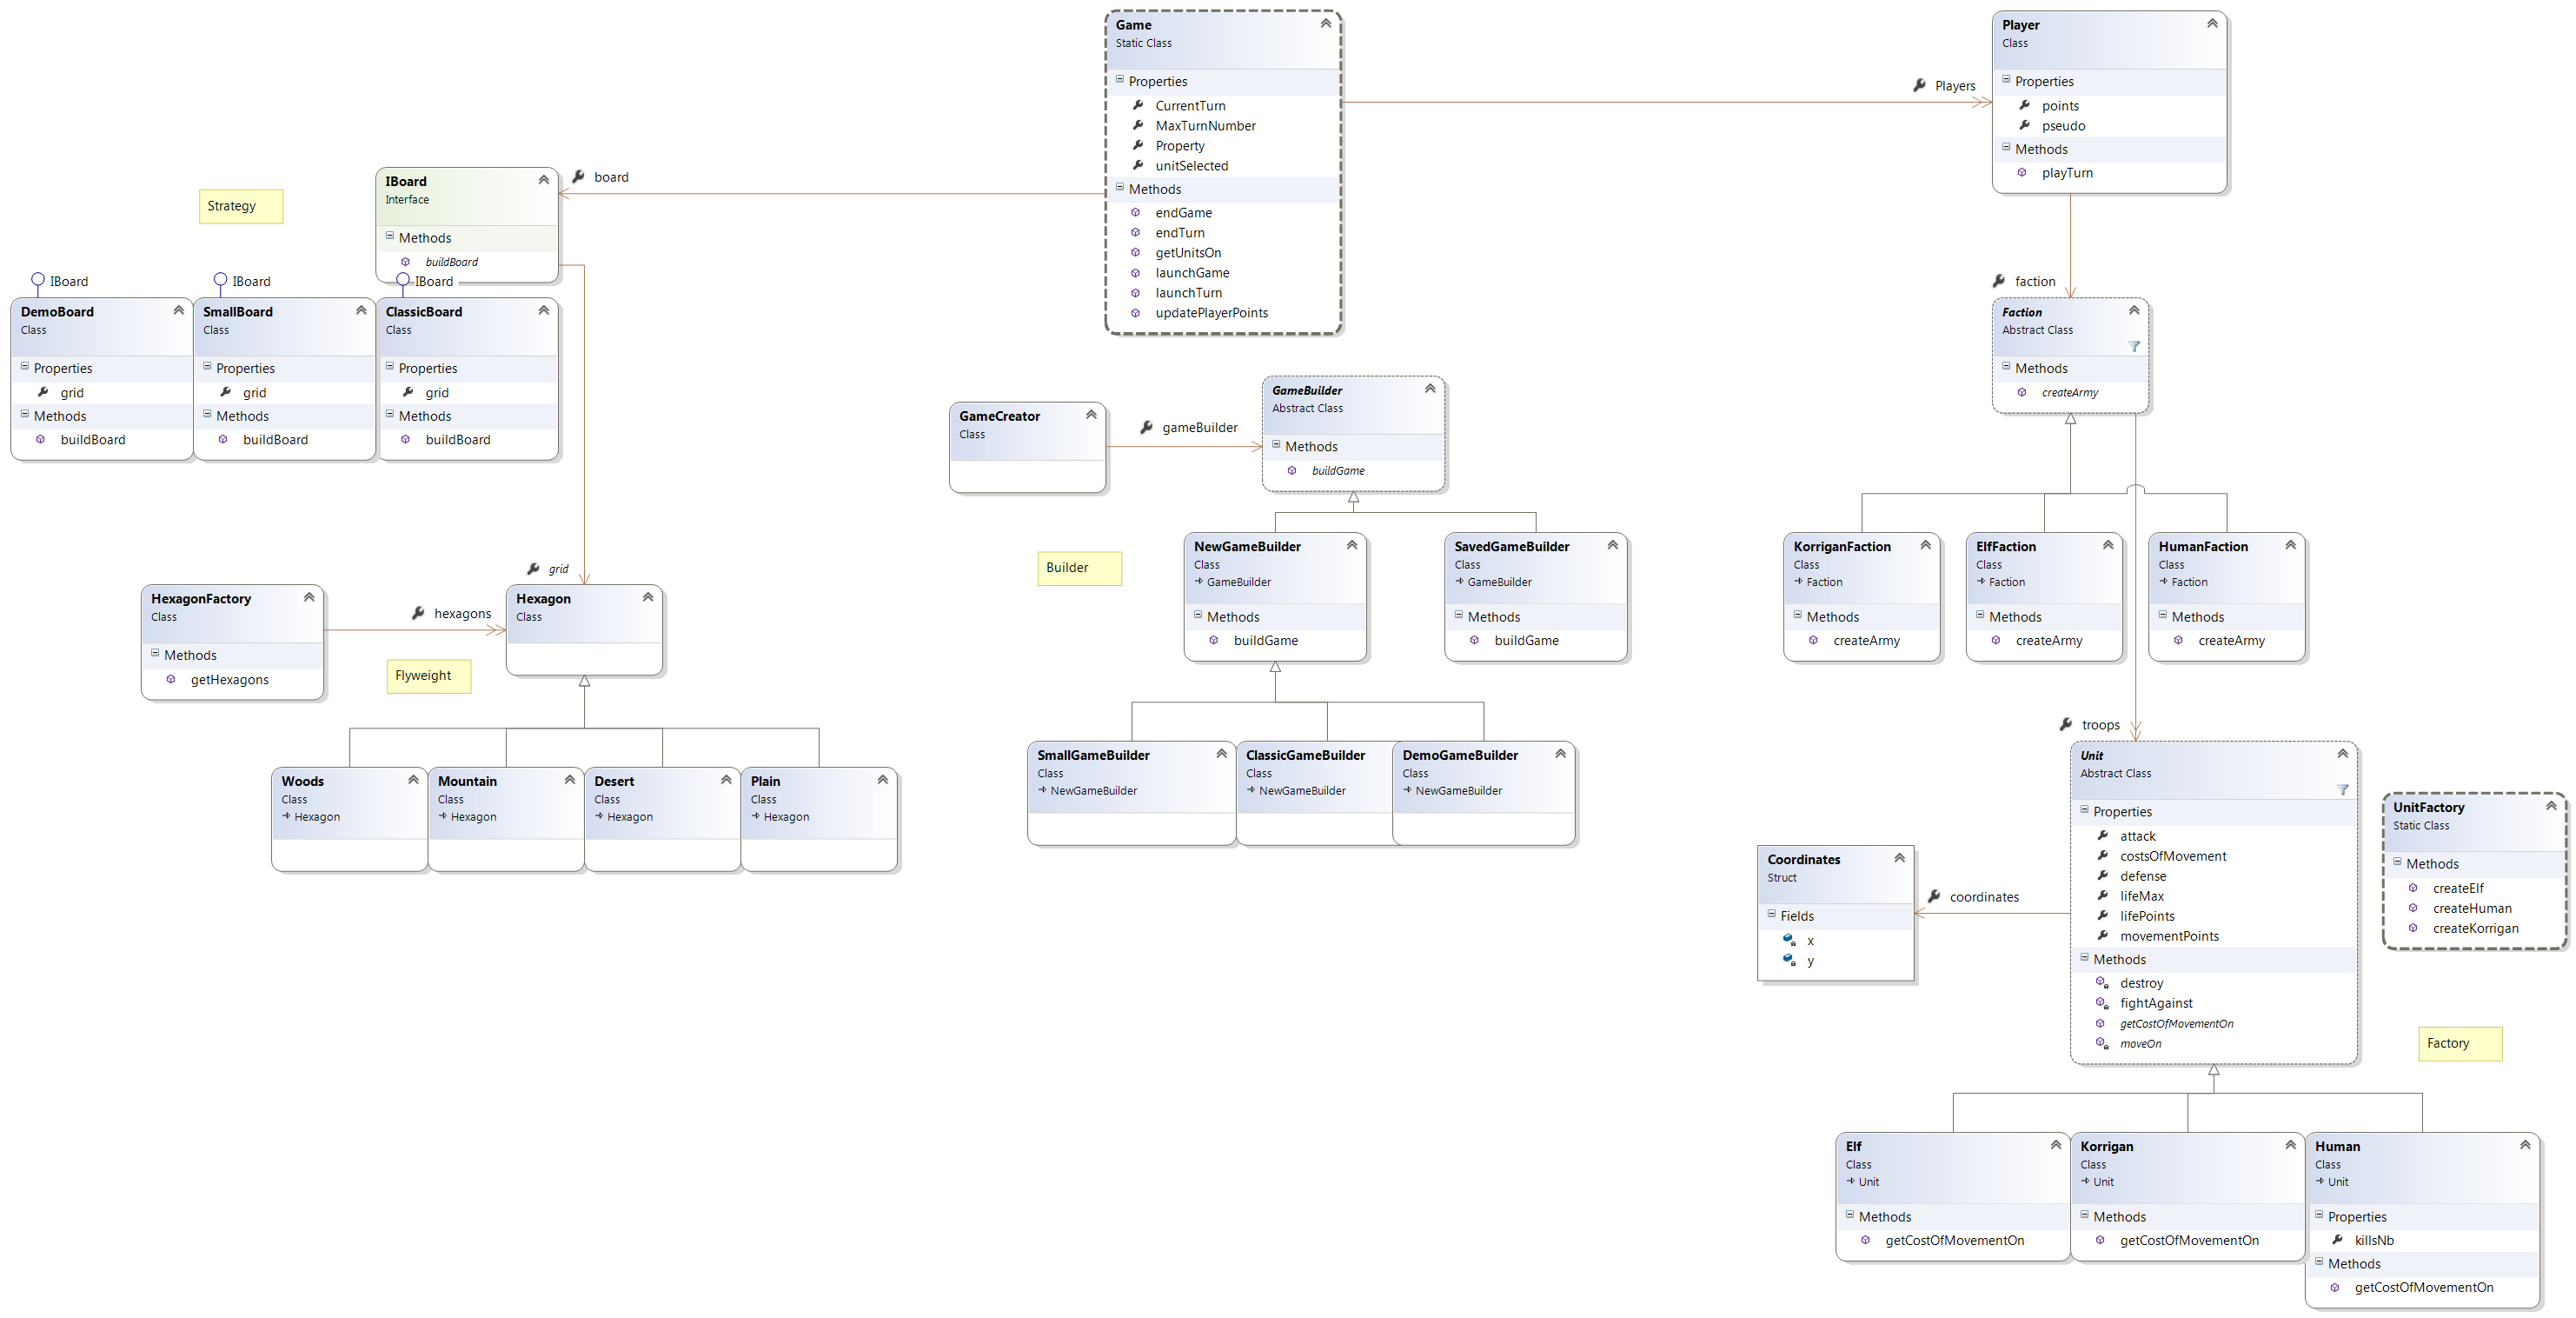
\includegraphics[width=0.5\textwidth]{figure/entire_class_diagram}
		\end{center}
		\caption{Diagrame de classe}
		\label{fig:planif}
	\end{figure}




